% From Felix Kwok, SCCM, Nov 30, 2007.
%
% Basically this is a template file -- you should be able to take it and
% start running.  It makes use of the suthesis-2e package from Emma Pease
%     http://help-csli.stanford.edu/tex/suthesis/

% The philosophy behind this template is that each chapter or
% chapterlike section goes in a separate file and you use the \include
% command to input it into the final document.  The \includeonly
% command can be used so you only need to work on one or two chapters
% at a time (instead of having to either latex the entire book each
% time or losing cross-references and page numbering)

% Copy this file and call it something like mythesis.tex

\documentclass[12pt,twsoside]{report}
% commands.tex
% Afra Zomorodian
% August 20, 2009
\usepackage{lineno}

%\usepackage[usenames,dvipsnames]{color}
%\usepackage{subfig}
\usepackage{amscd}
\usepackage{amsmath}
\usepackage{amsthm}
\usepackage{amssymb}
\usepackage{ifthen}
\usepackage{eucal} % for mathcal
\usepackage{url}
\usepackage{clrscode}
\usepackage{multirow}
\usepackage{graphicx}
\usepackage{proof}
\usepackage{times}
\usepackage{amsthm}
\usepackage{tikz}
\usepackage{tikz-cd}
\usepackage{epsfig}
\usepackage{subcaption}
\usepackage{shortlst}
%\usepackage{rotating}
%\usepackage{enumitem}
%\setlist{nolistsep}
\usepackage{multicol}
\usepackage{prelimdraft}
\usepackage{siunitx}
\setcounter{page}{0}

%% units are in inches
%\setlength{\unitlength}{1in}
%
%% Useful macros for graphics
%% centerfig
%\newcommand{\centerfig}[2]{%
%\centerline{\includegraphics[#2]{figs/#1}}
%}
%
%\newcommand{\boxedcenterfig}[2]{%
%%\setlength{\fboxsep}{0pt}
%\centerline{\fbox{\includegraphics[#2]{figs/#1}}}
%}
%
%\setlength{\fboxsep}{1pt}
%
%%% Define a new style for the package that will use a smaller font.
%\makeatletter
%\def\url@smallurlstyle{%
%  \@ifundefined{selectfont}{\def\UrlFont{\sf}}{\def\UrlFont{\small\ttfamily}}}
%\makeatother
%% Now actually use the newly defined style.
%\urlstyle{smallurl}
%
%% subimg
%\newcommand{\subimg}[5][-1]{%
%\subfigure[#5]{%
%  \label{#4}
%  \ifthenelse {\equal{#1}{-1}}
%    {\includegraphics[#3]{figs/#2}}
%    {\begin{minipage}[b]{#1\columnwidth}{%
%      \centerline{\includegraphics[#3]{figs/#2}}}
%    \end{minipage}
%    }
%}}
%
%% subimgnt
%\newcommand{\subimgnt}[3][-1]{%
%\subfigure{%
%  \ifthenelse {\equal{#1}{-1}}
%    {\includegraphics[#3]{figs/#2}}
%    {\begin{minipage}[b]{#1\columnwidth}{%
%      \centerline{\includegraphics[#3]{figs/#2}}}
%    \end{minipage}
%    }
%}}

% mathbb
\newcommand{\R}{\ensuremath{\mathbb{R}}}
\newcommand{\NN}{\ensuremath{\mathbb{N}}}
\newcommand{\Q}{\ensuremath{\mathbb{Q}}}
\newcommand{\Z}{\ensuremath{\mathbb{Z}}}
\newcommand{\F}{\ensuremath{\mathbb{F}}}
\newcommand{\emax}{\ensuremath{\hat{\epsilon}}}
\newcommand{\vr}{\ensuremath{\mathcal{V}}}
\newcommand{\vrs}{\ensuremath{\vr_{\epsilon}(S)}}
\newcommand{\es}{\ensuremath{E_{\epsilon}(S)}}
\newcommand{\vs}{\ensuremath{V_{\epsilon}(S)}}
\newcommand{\vrms}{\ensuremath{\vr_{\emax}(S)}}
\newcommand{\ges}{\ensuremath{G_{\epsilon}(S)}}
\newcommand{\gemax}{\ensuremath{G_{\emax}(S)}}
\newcommand{\weight}{\ensuremath{\omega}}
\newcommand{\gweight}{\ensuremath{w}}
\DeclareMathOperator{\dist}{d}
\newcommand{\cplusplus}{C\raisebox{0.5ex}{\small ++}}
\newcommand{\Filt}[1]{\ensuremath{\leq_{#1}}}

% names
\newcommand{\cech}{\v{C}ech} % not in math mode
\newcommand{\acm}{ACM}
\newcommand{\ieee}{IEEE}
\newcommand{\siggraph}{SIGGRAPH}
\newcommand{\etlsh}{\textsc{E\raisebox{0.7ex}{\scriptsize 2}LSH}}
\newcommand{\ann}{\textsc{Ann}}
\newcommand{\cgal}{\textsc{Cgal}}
\newcommand{\plex}{\textsc{Plex}}

%%complexity classes
\newcommand{\complexity}[1]{\textsc{#1}}
\newcommand{\NPH}{\complexity{NP-Hard}}
\newcommand{\NP}{\complexity{NP}}
\newcommand{\NPC}{\complexity{NP-Complete}}
\newcommand{\APX}{\complexity{APX}}
\newcommand{\APXC}{\complexity{APX-Complete}}

%%decision problems
\newcommand{\ablp}{\textsc{$\alpha$-Balanced-Minimum-Blowup}}
\newcommand{\dablp}{\textsc{Dual-$\alpha$-Balanced-Minimum-Blowup}}
\newcommand{\aedge}{\textsc{$\alpha$-Balanced-Edge-Separator}}
\newcommand{\avertex}{\textsc{$\alpha$-Subgraph-Balanced-Vertex-Separator}}
\newcommand{\aBMB}{\textsc{$\alpha$-Bmb}}
\newcommand{\aBES}{\textsc{$\alpha$-Bes}}
\newcommand{\aBVS}{\textsc{$\alpha$-Bvs}}
\newcommand{\YES}{\textsc{Yes}}

\newcommand{\scitem}{\textsc{\normalfont\item}}

% algorithms
\newcommand{\allpairs}{\proc{All-Pairs}}
\newcommand{\scan}{\proc{Scan}}
\newcommand{\kdexact}{\proc{Kd-Exact}}
\newcommand{\kdapprox}{\proc{Kd-Approx}}
\newcommand{\bbdexact}{\proc{BBD-Exact}}
\newcommand{\bbdapprox}{\proc{BBD-Approx}}
\newcommand{\witness}{\proc{Witness}}
\newcommand{\Foreach}{\textbf{foreach} }

% expansion
\newcommand{\inductive}{\proc{Inductive-VR}}
\newcommand{\incremental}{\proc{Incremental-VR}}
\newcommand{\maximal}{\proc{Maximal-VR}}
\newcommand{\lowerneighbors}{\proc{Lower-Nbrs}}
\newcommand{\addcofaces}{\proc{Add-Cofaces}}
\newcommand{\ikgx}{\proc{IK-GX}}
\newcommand{\generatecombinations}{\proc{Generate-Combinations}}
\newcommand{\computeweightfunction}{\proc{Compute-Weights}}
\newcommand{\computeweight}{\proc{Weight}}
\newcommand{\ceil}[1]{\left \lceil#1\right \rceil}
\newcommand{\floor}[1]{\lfloor#1\rfloor}

% data sets
\newcommand{\bunny}{{\textsf{B}}}
\newcommand{\sphere}{\textsf{S}}
\newcommand{\clique}{\textsf{C}}
\newcommand{\multiblob}{\textsf{M}}
\newcommand{\blobs}{\multiblob}
\newcommand{\gnp}{\textsf{G}}

% Erdos-Renyi
\newcommand{\Erdos}{Erd\H{o}s}
\newcommand{\Renyi}{R{\'e}nyi}
\newcommand{\almosta}{a.a.\@}

\renewcommand{\Im}[1]{\operatorname{Im}{#1}}
\newcommand{\Ker}[1]{\operatorname{Ker}{#1}}
%\newcommand{\rank}[1]{\operatorname{rank}{#1}}
\newcommand{\Dim}[1]{\operatorname{dim}{#1}}
\newcommand{\bd}{\ensuremath{\partial}}
\DeclareMathOperator{\im}{im}
\DeclareMathOperator{\size}{size}
\newcommand{\betti}{\ensuremath{\beta}}
\newcommand{\tensor}{\otimes}
\DeclareMathOperator{\rank}{rank}
\newcommand{\Bd}[1]{\partial_{#1}}
\newcommand{\Cl}[1]{\operatorname{Cl}{#1}}
\newcommand{\bigslant}[2]{{\raisebox{.2em}{$#1$}\left/\raisebox{-.2em}{$#2$}\right.}}
\newcommand{\card}[1]{|#1|}
\newcommand{\mv}{Mayer-Vietoris }
\newcommand{\mvb}{\mv blowup complex}
\newcommand{\K}{K}
\renewcommand{\L}{L}
\newcommand{\C}{U}
\newcommand{\N}{N}
\newcommand{\M}{M}
\newcommand{\factor}{\card{\K^{\C}}/\card{\K}}
\newcommand{\ratio}{\factor}
\newcommand{\Parfor}{\kw{parallel for}}
\newtheorem{theorem}{Theorem}
\newtheorem{lemma}{Lemma}
%\newtheorem{corollary}[theorem]{Corollary}
\newtheorem{corollary}{Corollary}[lemma]
\theoremstyle{definition}
\newtheorem{example}{Example}[subsection]
\newtheorem{fact}{Fact}[subsection]
\newtheorem{definition}{Definition}[section]

%%%%%%%%%%
%Afra's Colors
%%%%%%%%%
\definecolor{afra}{RGB}{198,168,208}
\definecolor{afrablue}{RGB}{143,166,215}
\definecolor{afragreen}{RGB}{182,215,112}
\definecolor{afrapurple}{RGB}{218,177,239}
\definecolor{darkgray}{gray}{0.3}
\definecolor{afrapurplelight}{RGB}{198,168,208}
\definecolor{afrabluedark}{RGB}{75,113,191}
\definecolor{afrabluelight}{RGB}{143,166,215}
\definecolor{afragreendark}{RGB}{154,191,75}
\definecolor{afragreenlight}{RGB}{182,215,112}
\definecolor{afrapurpledark}{RGB}{162,75,191}

\usepackage{xcolor}
\usepackage{pgfplots}
\usepackage{pgfplotstable}
\usepackage{filecontents}
\usetikzlibrary{calc, fit, shadows, arrows, positioning, patterns, external, matrix}
% if these lines are commented out, the box draws.
\pgfdeclarelayer{edges}
\pgfdeclarelayer{quadcell}
\pgfsetlayers{quadcell,edges,main}
\pgfplotsset{compat=newest}

%%%%%%%%%%%
%%BEGIN TIKZ TODO LOGIC
%%%%%%%%%%%%%%%
\makeatletter \newcommand \listoftodos{\section*{Todo list} \@starttoc{tdo}}
\newcommand\l@todo[2]
  {\par\noindent \textit{#2}, \parbox{10cm}{#1}\par} \makeatother

\newcommand{\todo}[1]{
% Add to todo list
\addcontentsline{tdo}{todo}{\protect{#1}}
%
\begin{tikzpicture}[remember picture, baseline=-0.75ex]
    \node [coordinate] (inText) {};
\end{tikzpicture}
%
% Make the margin par
    \begin{tikzpicture}[remember picture]
        \definecolor{orange}{rgb}{1,0.5,0}
 
        \draw node[draw=black, fill=orange, text width = 5cm] (inNote)
                 {#1};
    \end{tikzpicture}
%
%\begin{tikzpicture}[remember picture, overlay]
%    \draw[draw = orange, thick]
%        ([yshift=-0.2cm] inText)
%            -| ([xshift=-0.2cm] inNote.west)
%            -| (inNote.west);
%\end{tikzpicture}
%
}
\graphicspath{{figs/},{figs/speedup-figs/}}

\def\lbl#1#2{\begingroup
	    #2%
	    \def\@currentlabel{#2}%
	    \phantomsection\label{#1}\endgroup
	}

\input{data}
% Note that the documentclass can take other options such as
%   twoside - for double sided printing
%   openright - if double side  chapters always start on odd pages
%   openany - if double side chapters start on the next page even or odd
% 10pt can be replaced by 11pt (or 12pt), but NOTE THAT
% THE REGISTRAR'S OFFICE ACCEPTS THE PARAMETERS SHOWN HERE,
% including \setstretch{1.213}, which seems to be as close
% to single spacing as they allow so far (2007).

\usepackage{suthesis-2e}
\usepackage{amsmath, amsfonts, amsthm,
  verbatim, fancyhdr, graphicx, array,
  color, listings, afterpage, epsfig, boxedminipage}

%% Load other packages you need

%% Uncomment the following and create mythesis-macros.sty for all your
%% own macros.  This keeps this top level file looking fairly neat.
% \usepackage{mythesis-macros}

%% Certain types of theses require special title page format.  See the
%% style file for the full list.  An example would be that for some of
%% the language departments.
% \dualthesis \dept{Asian Languages} \languagemajor{Korean}
%% or educationhttps://www.facebook.com/danshaffer
% \educationthesis

   \title{Spectral Sequences and Applied Topology}
   \author{Ryan H. Lewis}
   \programthesis
   \dept{Institute for Computational and Mathematics and Engineering}
   \principaladviser{Gunnar Carlsson}
%  \coprincipaladvisor{}
   \firstreader{Leonidas Guibas}
   \secondreader{Jack Poulson}
  \thirdreader{Dmitry Morozov}

% The following command would (if uncommented) allow only
% chapter1 and chapter2 to be processed
% \includeonly{chapter1,chapter2}

% If you feel real savvy use
% \typein{Now put in includeonly}
% The \typein command stops latex at this point and allows you to type
% in a command such as
%    \includeonly{chapter3,chapter5}
% This can save some time and means you don't have to edit this file
% as much.

\setstretch{1.213}  % SAVE SOME TREES WITH THIS AND 10pt

\begin{document}

\maketitle
% First the preface sections.

% This includes the file preface.tex which should include the
% following commands
% \beforepreface
 \prefacesection{Abstract}
% body of the preface
%\include{abstract}
Shape matters for data analysis. In this thesis we investigate the utility of spectral sequences for persistent homology, a tool which characterizes the shape of data. We show how to compute p.h. in parallel. 

% Any other preface sections

% The last preface section (e.g., acknowledgement.tex)
% should look like
 \prefacesection{Acknowledgement}
This thesis could not have existed without my advisor Gunnar Carlsson. Without his mentorship I do not know where I would be. He has a unique ability to push people far beyond there mathematical comfort levels. I am grateful to Leonidas Guibas, Jack Poulson, Dmitry Morozov, and  for serving on my thesis committee. I would like to thank the Stanford Computational Topology group, whose lively meetings have taught me so much. Conversations with Anthony Bak, Michael Kerber, Michael Lesnick, and Pawin Vongmasa have shown me that creativity can get you quite far. Because of my friends in ICME including Austin Benson, Victor Minden, Bradley Nelson, Anil Damle, and Nolan Schodopole, I have many happy memories of my time in Graduate School. 

I am indebted to my soon to be wife, Elena, as well as my family for there patience and support.

% body
 \afterpreface
%\include{acknowledgement}


% Now for the body of the thesis, modify the number of these lines as
% needed

% This includes chapter1.tex which should start with a \chapter{...}
% command

\chapter{Introduction}
\begin{figure}
\centering
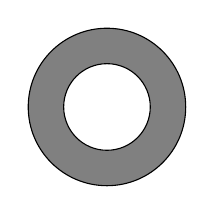
\begin{tikzpicture}[scale=.25]
  \filldraw[draw=black,fill=gray] (0,0) circle [radius=4];
      \filldraw[draw=black,fill=white] (0,0) circle [radius=2.2];
 \end{tikzpicture}      
 \hspace{.5cm}
\begin{tikzpicture}[scale=.25]
    \foreach[count=\p] \x / \y in \data { 
	\node[draw, circle, scale=.25, fill=white](\p) at (\x, \y) {};
    } 
 \end{tikzpicture}
 \caption{Point Cloud sampled from annulus}
 \end{figure}
Over the past twenty years \emph{topological data analysis} has been found to be very useful in understanding scientific data. The primary tools of the field: persistent homology and mapper have been used in image processing, chemistry, astronomy, business, and medicine. The dichotomy with traditional data analysis, in which one concerns itself with modeling physical phenomena from measurements on finite sets of samples, is that in topological data analysis, one assumes that the input point cloud comes from an unknown underlying geometric space. Topological data analysis then focuses on the recovery of the lost topology of this underlying space \cite{c-tnd-09}. In this thesis we aim to make the primary tool for topological data analysis, persistent homology, computable for practitioners. To this end we investigate parallel algorithms for the computation of persistent homology. We present two new parallel algorithms for persistence, the first for computing homology, and the second which extends it to the persistent setting. We connect these procedures to \emph{spectral sequences} a manual calculation tool used by mathematicians for computing algebraic structures by hand.
\section{Background}
Suppose someone asked you describe the shape of this point cloud. One might be inclined to propose that the point cloud looks quite disconnected. Indeed, the topology of a set of points in $\R^n$ is not all that interesting. Perhaps, however, if you were to squint your eyes, you might be inclined to describe the shape as something like an annulus. Persistence is a tool for modeling this phenomenon. As an example, for any \emph{metric space} $(X,d)$ and  $\epsilon > 0$ we can define a space: \[ M_\epsilon = \bigcup_{x \in X} B_{\epsilon}(x) \] where $B_{\epsilon}(x) = \{ y \mid d(x,y) < \epsilon\} $ is the \emph{ball of radius $\epsilon$ around x}. Notice that by varying the scale parameter $M_\epsilon$ has different topologies. The collection $\{M_\epsilon\}_\epsilon$ of spaces together with the inclusion maps between $M_\epsilon$ and $M_{\epsilon'}$ for any $\epsilon < \epsilon'$ is called a \emph{one parameter family} of spaces.   
 
 \begin{figure}
\centering
 \hspace{.5cm}
 \begin{tikzpicture}[scale=.25]
\begin{pgfonlayer}{ball}
      \foreach[count=\p] \x / \y in \data {
         \fill[gray!50,radius= .3 cm] (\x,\y) circle{};
	}
 \end{pgfonlayer}{ball}
	\foreach[count=\p] \x / \y in \data {
	 \node[draw, circle, scale=.25, fill=white](\p) at (\x, \y) {};
	 }
\end{tikzpicture}
 \hspace{.25cm}
\begin{tikzpicture}[scale=.25]
\begin{pgfonlayer}{ball}
      \foreach[count=\p] \x / \y in \data {
         \fill[gray!50,radius= .6 cm] (\x,\y) circle{};
	}
 \end{pgfonlayer}{ball}
	\foreach[count=\p] \x / \y in \data {
	 \node[draw, circle, scale=.25, fill=white](\p) at (\x, \y) {};
	 }
\end{tikzpicture}
 \hspace{.25cm}
\begin{tikzpicture}[scale=.25]
\begin{pgfonlayer}{ball}
      \foreach[count=\p] \x / \y in \data {
         \fill[gray!50,radius= 1 cm] (\x,\y) circle{};
	}
	\fill[gray!50,radius= 2.4 cm] (0,0) circle{};
 \end{pgfonlayer}{ball}
	\foreach[count=\p] \x / \y in \data {
	 \node[draw, circle, scale=.25, fill=white](\p) at (\x, \y) {};
	 }
\end{tikzpicture}
\caption{Model spaces at various scales}
\end{figure}

 Persistent topology concerns itself with topological features which can be found at multiple scales.

\section{Preliminaries}
We begin with a review of algebraic topology. 
We refer the reader to Hatcher for background material in algebraic topology~\cite{hatcher}.

A \emph{simplicial complex} is a collection $\K$ of finite sets called
\emph{simplices} such that if $\sigma \in \K$ and $\tau \subseteq \sigma$ then 
$\sigma \in \K$. We say that $\tau$ is a \emph{face} of $\sigma$, its \emph{coface}. A simplex
is \emph{maximal} if it has no proper coface in $\K$. The set of maximal cells of a 
simplicial complex $\K$ is $\M(\K)$. If $\card{\sigma} = k+1$
then $\sigma$ is a $k$-simplex, it has \emph{dimension} $k$, denoted 
$\dim{\sigma} = k$. We say that $\K$ is \emph{$d$-dimensional} if 
$d = \max_{\sigma \in \K} \dim{\sigma}$. 

Suppose we have a subset $L \subseteq K$.  $L$ is a \emph{subcomplex}
if it is a simplicial complex. The \emph{closure} of $L$ is 1
$\Cl(L) = \{ \tau \mid \tau \subseteq \sigma \in L\}$ and it is a simplicial complex. The 
\emph{$k$-skeleton} of a complex $\K$ is the set of all simplices
of dimension less than or equal to $k$. Note that the 1-skeleton of
any complex is as a graph.

Let $\Delta^n$ be the $n$-simplex defined on $[n+1]$.  We note that 
$\Delta^n$ is traditionally defined in a geometric setting and is
called the \emph{standard $n$-simplex}~\cite{hatcher}, although we 
are using an abstract version here for our purposes. For any
\emph{indexing set} $J \subseteq [n]$, $\Delta^J$ is the $(\card{J}-1)$ 
dimensional face of $\Delta^n$  that is defined on $J$.

We define a \emph{filtration} of topological spaces to be a finite sequence of topological spaces connected by
continuous maps. Given a filtration of simplicial complexes, whose final space is $\K$ we can create a  
partial ordering on the simplices of $\K$ such that the $i^{th}$ prefix of the ordering is the image in $\K$ of the $i^{th}$ map. Each prefix is itself a subcomplex of $\K$, so in practice we consider only filtrations of spaces connected by inclusion maps.

Given a simplicial complex $\K$, An \emph{open cover} of $\K$ is a collection of subsets $\{C_i\}_i$ of $\K$ where the union of the $C_i$ is $\K$. Similarly, we call a cover closed if each element of the cover is a subcomplex. 

The \emph{nerve} $\N(\C)$ of a cover $\C$ is the simplicial complex on $[\card{\C}-1]$ whose $k$-simplices 
represent the non-trivial intersections of subsets of $\C$ of size $k+1$. The nerve is a subcomplex of the standard $n$-simplex and so we may denote its simplices by $\Delta^J$ where $J \subseteq [\card{\C}-1]$. 

It is sometimes convenient to encode the cover $\C$ as a map $N: \K \rightarrow \Delta^[\card{\C}]$ where each 
simplex $\sigma \in \K$ is mapped to the list of the cover sets containing $\sigma$.

A simplicial complex may be viewed as the result of gluing simplices of 
different dimensions along common faces. Other types of complexes are defined 
similarly using different types of \emph{cells}. Such \emph{cellular} complexes include \emph{cubical} complexes, \emph{simplicial sets}. $\Delta$-complexes, and \emph{CW-complexes}, 
to name a few~\cite{ez-ssc-50,hatcher,kmm-ch-04,m-soat-68}. 

\section{Homology}
In this section, we describe the homology of cellular spaces over 
field coefficients. Homology, however, is an invariant of arbitrary topological 
spaces and may be computed over arbitrary coefficient rings~\cite{hatcher}.  
Suppose we are given a finite cellular complex $\K$ and a field $k$. 
The \emph{$n$th chain vector space $C_n$} is the $k$-vector space generated by 
the set of $n$-dimensional cells of $K$, its \emph{canonical basis}.  
Suppose we are given a linear \emph{boundary operator} 
$\bd_n\colon C_n \rightarrow C_{n-1}$ such that 
$\bd_n \circ \bd_{n-1} \equiv 0$ for any $n$.  
The boundary operator connects the chain vector space into a 
\emph{chain complex $C_*$}:
\begin{equation*}
  \cdots \rightarrow             C_{n+1}
         \xrightarrow{\bd_{n+1}}  C_n
         \xrightarrow{\bd_n}     C_{n-1}
         \rightarrow \cdots .
\label{eqn:chaincomplex}
\end{equation*}
Given any chain complex, the \emph{$n$th homology vector space $H_n$} is:
\begin{equation}
  \label{eqn:homology}
  H_n = {\ker{\bd_n}}\,/\,{\im{\bd_{n+1}}}, 
\end{equation}
where $\ker(.)$ and $\im(.)$ are the \emph{kernel} and \emph{image} of $\bd$, 
respectively.
Each homology vector space is characterized fully by its \emph{Betti number}, 
$\betti_n = \dim{H_n}$.  
We now only need to define boundary operators to get homology. 
For simplicial homology, we begin by defining the action of the boundary operator on any
$n$-simplex $[v_0,\ldots,v_n] \in \K$:

\begin{equation*}
\bd_n [v_0,\ldots,v_n] = \sum_i (-1)^i [v_0,\ldots,\hat{v_i},\ldots,v_n],
\end{equation*}
where $\hat{v_i}$ indicates that $v_i$ is deleted from the vertex 
sequence. The boundary operator is the linear extension of the above action.

Over field coefficients, homology is a vector space characterized by its dimension, 
so we may compute homology using \emph{Smith Normal Form}~\cite{uhlig}, a matrix reduction technique 
similar to Gaussian Elimination~\cite{uhlig}. However, because we reduce boundary matrices and not general matrices, we may perform specific optimizations to improve the practical running time of these procedures. 
The original modified algorithm is referred to as the persistence algorithm~\cite{elz-tps-02,zc-cph-05}. 
\section{Persistent Homology}

\chapter{Filtrations \& Persistent Homology}
In this chapter we will define persistent homology, and provide some algorithms for computing them. Suppose we have a one parameter family of  $X = \{ X_\alpha \}$ of topological spaces. For example, consider the one parameter family of Cech complexes computed from the model spaces in Figure~\ref{model-spaces}. Observe that there is some minimal scale $\alpha$ at which the major cycle of the annulus appears. Further, at some later scale $\beta$, this cycle becomes the boundary of a higher dimensional $2$-chain. In other words if we refer to the cycle as $c$, then $[c] \in \Im(\partial_2(X_\beta))$. This type of data is what is referred to as persistent homology. To make this more formal, recall that the one parameter family of $X$ gives rise to a one-parameter family of homology vector spaces in dimension $d$, connected by induced linear maps. We may associate to this one parameter family a graded $k[t]$-module \[ H(X) := \bigoplus_\alpha t^i H(X_\alpha) \] called the \emph{persistent homology module}. The action of the indeterminate $t$ on an element in $H(X_\alpha)$ is defined by applying the induced linear map $f_\alpha$. It is possible to characterize the lifetime of all the elements in the persistent homology module. That is, module elements are born (appear) at particular grades, and may exist as a nontrivial element until a later grade, when it becomes the boundary of some higher dimension surface. It turns out that when persistent homology is computed over field coefficients one can systematically organize the elements of the persistent homology module by this lifetime information. 
\begin{theorem} Let $H(X) = \bigoplus_\alpha t^\alpha H(X_\alpha)$ be a graded $k[t]$-module for some field $k$. Then we have that 
\[ H(X) \simeq \left( \bigoplus_{\alpha_i}t^{\alpha_i}R[t] \right) \bigoplus \left( \bigoplus_{[\alpha_i, \beta_i]} t^{\alpha_i}R[t]/t^{\beta_i}  \right)  \]
The collection of intervals $[\alpha_i,\beta_i]$ together with the intervals $[\alpha_i, \infty)$ are a complete and discrete invariant 
of the module $\K$. 
\end{theorem}
\begin{proof}
Carlsson \& Zomorodian~\cite{zc-cph-04}.
\end{proof}
The collection of intervals is referred to as a barcode. In the next section we make use of a \emph{spectral sequence} to decompose $H(X)$ into its invariant form. This exposition allows us to derive persistent homology constructively, using only linear algebra. It also lends itself to deriving \emph{the persistence algorithm}, and provides it's correctness proof. This connection of persistent homology to spectral sequences is not new~\cite{zc-cph-04}, however there does not seem to be any source which proves this relationship. A spectral sequence is a sequence of chain complexes $(E_i, d_i)$ called \emph{pages}. The elements of $E_i$ are referred to as \emph{terms}, and the operators $d_i$ are referred to as \emph{differentials}. The terms on page $E_{i+1}$ are defined to be the homology of the chain complex on the previous page.

\section{The Spectral Sequence of a Filtration}
The \emph{spectral sequence of a filtration} generalizes the long exact sequence of a pair, to the case of a filtration.

Let $R$ be a commutative ring and $0 \rightarrow \K_0 \rightarrow \K_1 \rightarrow  \ldots \rightarrow  \K_n$ 
be a filtration of chain complexes so that \[ \K_i = C_*(X_i, R) = \bigoplus_d C_d(X_i, R)\] is a free $R$-module.
\[ \K = \bigoplus_i \K_i \] is a graded $R[t]$-module.

\noindent We begin with the original filtration of $\K$
\[
\begin{tikzcd} [column sep=small]
0 \arrow{r}{i} & \K_0 \arrow{r}{i} & \K_1 \arrow{r}{i}   & \K_2 \arrow{r}{i} & \ldots \arrow{r}{i} & \K_{n-1} \arrow{r}{i} & \K_n
\end{tikzcd}
\]
We refer to the homology of this sequence as the $E_0$ page of the spectral sequence. Next, we demonstrate how to construct the $E_1$ page.

\noindent With each map $K_i \rightarrow K_{i+1}$ we get a short exact sequence by attaching the cokernel:
\[
\begin{tikzcd} [column sep=small]
0 \arrow{r}{i} & \K_0 \arrow{r}{i}\arrow{d}{j} & \K_1 \arrow{r}{i}\arrow{d}{j}   & \K_2 \arrow{r}{i}\arrow{d}{j} & \ldots \arrow{r}{i} & \K_{n-1} \arrow{r}{i} \arrow{d}{j} & \K_n\arrow{d}{j} \\ 		&     \K_0/{0} &			 \K_1/{\K_0} & 	 \K_2/{\K_{1}}		   & \ldots  			   & \K_{n-1}/{\K_{n-2}}		 & \K_n/{\K_{n-1}} 
\end{tikzcd}
\]
This diagram passes to homology, where each short exact sequence extends to a long exact sequence. In the diagrams below denote the [relative] homology as the $k$-vector space which is the direct sum of homology computations in each dimension. Please keep in mind that the diagram below is not commutative, however each triangle is exact, and maps remain graded. Finally, we drop most indices on maps for visual clarity.
\[
\begin{tikzcd}[column sep=small]
0 \arrow{r}{i} & H(\K_0 \arrow{r}{i}\arrow{d}{j}) & H(\K_1 \arrow{r}{i}\arrow{d}{j})   & H(\K_2 \arrow{r}{i}\arrow{d}{j}) & \ldots \arrow{r}{i} & H(\K_{n-1}) \arrow{r}{i} \arrow{d}{j} & H(\K_n\arrow{d}{j}) \\ 		
&     H(\K_0) &			\arrow{l}{d_{1}} \arrow{ul}{\delta}  H(\K_1, {\K_0}) & 	\arrow{l}{d_{1}} \arrow{ul}{\delta} H(\K_2, {\K_{1}})		   & \arrow{l}{d_{1}} \arrow{ul}{\delta} \hspace{.5cm} \ldots  			   &\arrow{l}{d_{1}}\arrow{ul}{\delta}H(\K_{n-1}, {\K_{n-2}})		 & \arrow{l}{d_{1}} \arrow{ul}{\delta} H(\K_n, {\K_{n-1}})
\end{tikzcd}
\]
The terms of the $E_1$ page are defined as follows $E_{1,i} = H(K_i, K_{i-1})$.  The first differential $d_{1,i}: E_{1,i} \rightarrow E_{1,{i-1}}$ by $d_1 = j \circ \delta$. Now it remains to show that $(E_1, d_1)$ is a chain complex.
\begin{lemma} $d_1 \circ d_1 = 0$ \end{lemma} 
\begin{proof}
$d_1 \circ d_1 = (j \circ \delta) \circ (j \circ \delta) = j \circ \overbrace{(\delta \circ j)}^{\textrm{exactness}} \circ\, \delta = 0.$
\end{proof}
To write the terms on the $E_{n+1}$ page of the spectral sequence we compute homology of the $E_{n}$ page. 
That is $E_{n+1} = H(E_n)$. 
The differentials on each page are then defined as follows:
\begin{definition} For $n > 0$ define $d_n = j \circ \overbrace{i^{-1} \circ \ldots \circ i^{-1}}^{(n-1)\textrm{ times}} \circ\, \delta$
\end{definition}
That $d_{n+1}$ is well defined follows from the fact that the terms on the $(n+1)^{st}$ page is the homology of the previous page. For example, to show that $d_2$ is well defined we need to show that $\delta([x]) \in \Im(i)$ for any $[x] \in E_{2,r}$ However we know that $d_1([x]) = 0$ by the construction of the $E_2$ terms, so in other words $\delta([x]) \in \Ker{(j)}$ and so by exactness $\delta([x]) \in \Im(i)$. A similar arguments holds on all higher pages.

As an example lets compute the spectral sequence for this filtration of spaces.
\begin{example}
\[ \textrm{pt} \rightarrow S^1 \rightarrow S^1 \rightarrow \ldots \rightarrow D^1 \] 
\end{example}
In the following diagram each row contains the terms on a given page of the spectral sequence
\begin{tikzcd}
\end{tikzcd}

\begin{example}
\[ \textrm{pt} \rightarrow S^1 \rightarrow S^1 \rightarrow \ldots \rightarrow S^2 \] 
\end{example}
\begin{tikzcd}
\end{tikzcd}
What we can see is that that the $E_\infty$ page of the spectral sequence contains represents $H(D^1)$. There is also an obvious $k[t]$-module structure on $E_\infty$. In particular that is: $E_\infty = \bigoplus t^j E_{\infty,j}$. However, we originally wanted to show that this construction produced the invariant decomposition of the persistent homology module. It turns out that we have already done that. Along the way to the $E_\infty$ page we actually have computed the persistence homology of the filtration itself. Specifically we build an \emph{associated graded complex} $H(K) = E_\infty \oplus \bigoplus_p H_p(K)$ where $H_p(K) = \bigoplus_r t^r \Im(d_{p,r}) / t^{r+p} \bigoplus E_\infty$. Note that the term associated graded complex is used differently in other contexts.
\begin{theorem}
For any field $F$ the persistent homology module $H(K,F)$ is isomorphic to $H(K)$.
\end{theorem}
\begin{proof}
We know that since $F$ is a field $H(K,F)$ can be decomposed. It remains to show that and indecomposable $I_{[b,d]}$ appears on page $p = (d-b)$. Take any representative cycle $x$ and let $x = \partial(y)$ such that $y$ appears in the filtration at index $d$. Observe that $[x] \notin E_{p,k}$ for $k < b$. For $b < k < d$ Observe that $[x]  = [0]$ for $[x] \in E_{p,k}$  since each term $E_{p,k}$ can viewed as a sub quotient of $E_{1,k} = H(X_k, X_{k-1})$ and since $[x] \in X_{k-1}$ then we can say that $[x] = [0] \in E_{1,k} $. It follows that for $[x] \in E_{p,k}$ that $[x] = [0]$. Therefore $d_l([y]) = 0$ for all $l < p$, and $d_p([y])=[x]$. So it follows that $H_p$ encodes all length p summands of $H(K,F)$.
\end{proof}
\section{The Spectral Sequence Algorithm}
\label{sec:persistence-algorithm}
Recall from Chapter 1, that computing ordinary homology with field coefficients is equivalent to gaussian elimination therefore writing $\partial_k$ as a matrix, we may employ the following procedure.

Observe that we may reduce the matrices in each dimension independently.
The spectral sequence of a filtration suggests an iterative approach to computing persistent homology in which at iteration $p$ the barcode of length at most $p$ is resolved. The following algorithm summarizes this construction.
%\begin{figure}
%\begin{codebox}
%\Procname{\proc{SS}($\partial$, K_1, \ldots K_m)}
%\begin{algorithm}
%\li \For{ p \gets 1 \ldots m}
%\li \For { r \gets p \ldots m}
%\li \ParFor
%\li R_p, U_p \gets \proc{ELZ}(\partial[ , ])
%\li \textsc{ Emit persistence pairs in R_p}
%\li \partial(0:K_{p-1},K_p) \gets  \partial(0:K_{p-1}, K_p)*U_p
%\End
%\end{algorithm}
%\end{figure}
This algorithm is stated in Figure~\ref{alg:ss-alg}. However, it is important to note the following facts:
\begin{enumerate}
\item When moving from page $p$ to page $p+1$ distinct differentials on the $p^{th}$ page may be reduced completely independently. 
\item The optimizations stated in the standard persistence algorithm may now be combined.
\end{enumerate}
This was recently written down by Bauer et. al~\cite{bkr-cccph-13}. We summarize these results.
\begin{theorem}
Any rows of a boundary matrix, which correspond to an elementary simplex $\sigma$ whose insertion did not generate a new cycle, may be dropped.
\end{theorem}
\begin{proof}
As we move from page $p$ to page $p+1$ we quotient by the elements of $\Im(d_p)$. Therefore, in all future differentials the co-domain of the map does not need to contain a basis element for any member of $\Im(d_p)$.
\end{proof}
This is sometimes referred to as the \emph{compressing} optimization~\cite{bkr-cccph-13}. In addition, we see that in order for a pairing to occur, we must eventually match a cycle in the kernel of a differential to a later element which has this cycle as it's boundary. This statement is extremely powerful in terms of computation of persistence. In other words, we know that $\bd(\bd(\sigma)) = 0$, and as such we know that the first term on the first page spectral sequence, which first contains, $\bd(\sigma)$, which is the same as the largest filtration index to contain any member of $\bd(\sigma)$, must contain $\bd(\sigma)$ in it's kernel. This knowledge allows us to short circuit significant computation. It is not difficult to see that these techniques can be used together by taking advantage of the previously described parallelism. The authors provide an algorithm with complexity $O(foobarbaz)$. 

This is not the only method for computing persistent homology in parallel. Many times extra information, in the form of a cover on a space, is available while computing persistence. It is natural to try and glue the local connectivity data of a cover together to provide the persistent homology of the entire filtration. Classically the mayer vietoris sequence is used for this purpose.
  
\chapter{The Mayer Vietoris Spectral Sequence}

%\section{Blowup Complex}
\begin{figure*}
\begin{subfigure}[t]{.33\textwidth}
\centering
%\hspace*{-1cm}%
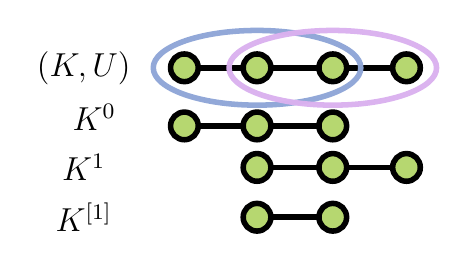
\begin{tikzpicture}[scale=.5, y=0.6pt, x=.75pt]
     %row 1
     \node[font=\large] at (-50, 800) {$(K, U)$};
     \draw[fill=afragreen, draw = black,  line width=2]  (47,800) circle (10pt);  
     \draw[fill=afragreen, draw = black, line width=2]  (117,800) circle (10pt);   
     \draw[fill=afragreen, draw = black, line width=2]  (190,800) circle (10pt); 
     \draw[fill=afragreen, draw = black, line width=2]  (261,800) circle (10pt); 
     \begin{pgfonlayer}{edges}
            \path[draw=black,fill=black,line width=2] (47,800) -- (117, 800);
            \path[draw=black,fill=black,line width=2] (117,800) -- (190, 800);
            \path[draw=black,fill=black,line width=2] (190,800) -- (261, 800);
      \end{pgfonlayer}      
      \draw[draw, color=afrablue, fill=none, line join=round,draw opacity=0.978,line width=2] (117, 800) ellipse (100 and 45);
      \draw[draw, color=afrapurple, fill=none, line join=round,draw opacity=0.978,line width=2] (190, 800) ellipse (100 and 45);
         %row 2 
    \node[font=\large] at (-40, 740) {$K^0$};
     \draw[fill=afragreen, draw = black, line width=2]  (47,730) circle (10pt);  
     \draw[fill=afragreen, draw = black, line width=2]  (117,730) circle (10pt);   
     \draw[fill=afragreen, draw = black, line width=2]  (190,730) circle (10pt); 
     \begin{pgfonlayer}{edges}
            \path[draw=black,fill=black,line width=2] (47,730) -- (117, 730);
            \path[draw=black,fill=black,line width=2] (117,730) -- (190, 730);
      \end{pgfonlayer}   
               %row 3
     \node[font=\large] at (-50, 680) {$K^1$};
     \draw[fill=afragreen, draw = black, line width=2]  (117,680) circle (10pt);   
     \draw[fill=afragreen, draw = black, line width=2]  (190,680) circle (10pt); 
      \draw[fill=afragreen, draw = black, line width=2]  (261,680) circle (10pt); 
         \begin{pgfonlayer}{edges}
            \path[draw=black,fill=black,line width=2] (117,680) -- (190, 680);
            \path[draw=black,fill=black,line width=2] (190,680) -- (261, 680);
      \end{pgfonlayer}   
          %row 4
\node[font=\large] at (-50, 620) {$K^{[1]}$};
     \draw[fill=afragreen, draw = black, line width=2]  (117,620) circle (10pt);   
     \draw[fill=afragreen, draw = black, line width=2]  (190,620) circle (10pt); 
         \begin{pgfonlayer}{edges}
            \path[draw=black,fill=black,line width=2] (117,620) -- (190, 620);
      \end{pgfonlayer}     
\end{tikzpicture}
\caption{Space and Cover}
\label{fig:space-n-cover}
\end{subfigure}
%\hfill
\begin{subfigure}[t]{.33\textwidth}
\centering
%	\def\svgwidth{1in}
%	\input{figs/local_pieces.pdf_tex}
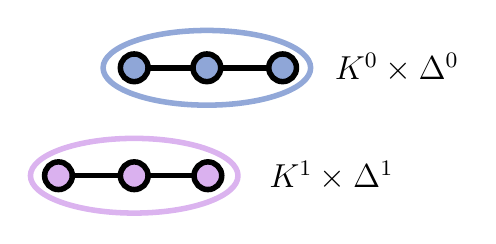
\begin{tikzpicture}[scale=.5, y=0.6pt, x=.75pt]
    %disj 0
    \begin{scope}[shift={(143,80)}]
    \node[font=\large] at (300, 730) {$K^0 \times \Delta^{0}$};
     \draw[draw, color=afrablue, fill=none, line join=round,draw opacity=0.978,line width=2] (117, 730) ellipse (100 and 45);
     \draw[fill=afrablue, draw = black, line width=2]  (47,730) circle (10pt);  
     \draw[fill=afrablue, draw = black, line width=2]  (117,730) circle (10pt);   
     \draw[fill=afrablue, draw = black, line width=2]  (190,730) circle (10pt); 
     \begin{pgfonlayer}{edges}
            \path[draw=black,fill=black,line width=2] (47,730) -- (117, 730);
            \path[draw=black,fill=black,line width=2] (117,730) -- (190, 730);
      \end{pgfonlayer}   
      \end{scope}
      %disj  1
       \begin{scope}[shift={(0,0)}]
         \node[font=\large] at (380, 680) {$K^1 \times \Delta^{1}$};
       \draw[draw, color=afrapurple, fill=none, line join=round,draw opacity=0.978,line width=2] (190, 680) ellipse (100 and 45);
     \draw[fill=afrapurple, draw = black, line width=2]  (117,680) circle (10pt);   
     \draw[fill=afrapurple, draw = black, line width=2]  (190,680) circle (10pt); 
      \draw[fill=afrapurple, draw = black, line width=2]  (261,680) circle (10pt); 
         \begin{pgfonlayer}{edges}
            \path[draw=black,fill=black,line width=2] (117,680) -- (190, 680);
            \path[draw=black,fill=black,line width=2] (190,680) -- (261, 680);
      \end{pgfonlayer}   
            \end{scope}
\end{tikzpicture}
\caption{Local pieces of the blowup complex.}
	\label{fig:local-pieces}
\end{subfigure}
%\hfill
\begin{subfigure}[t]{.33\textwidth}
\centering
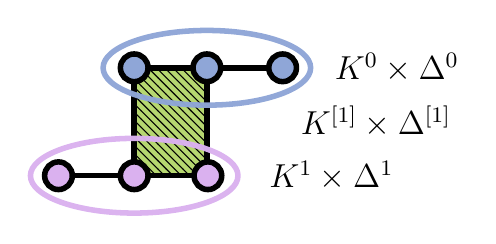
\begin{tikzpicture}[scale=.5, y=0.6pt, x=.75pt]
    %disj 0
    \begin{scope}[shift={(143,80)}]
    \node[font=\large] at (300, 730) {$K^0 \times \Delta^{0}$};
     \draw[draw, color=afrablue, fill=none, line join=round,draw opacity=0.978,line width=2] (117, 730) ellipse (100 and 45);
     \draw[fill=afrablue, draw = black, line width=2]  (47,730) circle (10pt);  
     \draw[fill=afrablue, draw = black, line width=2]  (117,730) circle (10pt);   
     \draw[fill=afrablue, draw = black, line width=2]  (190,730) circle (10pt); 
     \begin{pgfonlayer}{edges}
            \path[draw=black,fill=black,line width=2] (47,730) -- (117, 730);
            \path[draw=black,fill=black,line width=2] (117,730) -- (190, 730);
      \end{pgfonlayer}   
      \end{scope}
      %disj  1
       \begin{scope}[shift={(0,0)}]
         \node[font=\large] at (380, 680) {$K^1 \times \Delta^{1}$};
       \draw[draw, color=afrapurple, fill=none, line join=round,draw opacity=0.978,line width=2] (190, 680) ellipse (100 and 45);
     \draw[fill=afrapurple, draw = black, line width=2]  (117,680) circle (10pt);   
     \draw[fill=afrapurple, draw = black, line width=2]  (190,680) circle (10pt); 
      \draw[fill=afrapurple, draw = black, line width=2]  (261,680) circle (10pt); 
         \begin{pgfonlayer}{edges}
            \path[draw=black,fill=black,line width=2] (117,680) -- (190, 680);
            \path[draw=black,fill=black,line width=2] (190,680) -- (261, 680);
      \end{pgfonlayer}   
            \end{scope}
      %blowup edges 
      \begin{scope}[shift={(143,80)}]
     \begin{pgfonlayer}{edges}
            \path[draw=black,fill=black,line width=2] (47,730) -- (47, 600);
            \path[draw=black,fill=black,line width=2] (117,730) -- (117, 600);
      \end{pgfonlayer}     
          \node[font=\large] at (280, 665) {$K^{[1]} \times \Delta^{[1]}$};
        \begin{pgfonlayer}{quadcell}
      \draw [fill=afragreen,  preaction={fill, afragreen}, pattern=north west lines, pattern color=black] (47, 600) rectangle (117, 730);
	\end{pgfonlayer}
	\end{scope}
\end{tikzpicture}
		\caption{The blowup complex.}
		\label{fig:blowup}
\end{subfigure}
\caption{Our approach. We are given a space equipped with a 
	 cover~(\protect\subref{fig:space-n-cover}), the former represented by a path with
         four vertices and three edges and the latter represented by ovals.  
	 First, at time $(t = 0)$ we blowup up the space into 
	 local pieces~(\protect\subref{fig:local-pieces}), each local piece is a copy of 
	 the corresponding cover set, then, at $(t = 1)$ we glue together 
	 duplicated simplices by adding in the blowup cells, rendering them 
	 homologically equivalent, which gives us the blowup 
	 complex~(\protect\subref{fig:blowup}).
}
\label{fig:vignette}
\end{figure*}

Like homology, the blowup complex may be defined for arbitrary topological 
spaces~\cite{zc-lh-08}, but in this paper we focus on blowups of simplicial 
complexes. For a longer exposition of the \mvb{} we refer the reader to Zomorodian
\& Carlsson~\cite{zc-lh-08}. Given a simplicial complex $K$ and cover 
$\C = \{\C_i\}_i$ of $n$ subcomplexes, let 
$\K^J = \bigcap_{k \in J} \C_j$. The \emph{Mayer-Vietoris blowup complex} is:
\begin{linenomath*}
\begin{align*}
\K^\C &= \bigcup_{\emptyset \not = J \subseteq [n-1]} \K^J \times \Delta^J,
\end{align*}
\end{linenomath*}
where $\times$ is the Cartesian product~\cite{zc-lh-08} and $\Delta^J$ is a face of $\N(\C)$. 

 % Do example here before any further talk.
\begin{example}
\label{ex:blowup}
Suppose we have a space $\K$ with cover $\C = \{ \C_0, \C_1 \}$ as is shown on 
the top of Figure~(\ref{fig:space-n-cover}), where we use a line as a 
representative space and ovals to indicate cover sets, and the four vertices
of the line are labeled from left to right as $a, b, c, d$ respectively.
The cover defines the intersection $\K^{[1]} = \K^{ \{ 0 , 1 \} }$. 
The corresponding blowup is shown in in Figure~(\ref{fig:blowup}). We list each of
the relevant pieces of $\K^{\C}$ as well as the nerve of the cover where we denote simplices as strings for 
brevity.  
\begin{linenomath*}
\begin{align*}
\N(\C) &= \{ 0, 1, 01 \} \\
\K^0 \times \Delta^{\{0\}} &= \{a,b,c,ab,bc\} \times \{0\}, \\
\K^1 \times \Delta^{\{1\}} &= \{b,c,d,bc,bd\} \times \{0\}, \\
\K^{[1]} \times \Delta^{[1]} &=\{b,c,bc\} \times \{01\}. 
\end{align*}
\end{linenomath*}
\end{example}

% simplicial
While we may then triangulate the blowup complex to get a simplicial complex in order 
to compute its homology, this is computationally prohibitive, due to the need for triangulation. 
Luckily this approach is also not necessary. To compute the homology of the blowup complex, we may interpret the definition 
above in another way.  At the space level, we may view each cell of the blowup complex as a product 
of two simplices $\sigma \times \tau$, where $\sigma \in \K$ and $\tau \in \N(\C) \subseteq \Delta^{[n]}$.  
For example, the product of two edges, $bc \times 01$, gives us a quadrilateral cell in Example~\ref{ex:blowup}.  
That is the definition specified is an example of a cellular complex. 
\begin{lemma}
$\K^\C$ is a CW-Complex
\end{lemma}
\begin{proof}
Recall from Lemma~\ref{lem:simp-is-cw} that any simplicial complex is a CW-complex. Any so by Lemma~\ref{lem:cw-complex-product} $\K^\C$ is a subset of the CW complex: $\K \times \Delta^\card{\C}$. We need to only verify that it is closed. This follows since if $\sigma \times \tau \in \K^\C$ then $\sigma \in \cap_{v \in \tau} \C_{v}$ So therefore $\sigma \in \cap_{v \in \rho} \C_v$ for any $\rho \subset \tau$. Similarly since each cover set is closed if $\alpha$ is a face of $\sigma$ then $\alpha \times \tau \in \K^\C$.  Therefore $\sigma \times \rho \in \K^\C$. So therefore $\K^\C$ is a CW-Complex.
\end{proof}

% key property
Our work is based on the following key property.
The blowup complex $\K^\C$ has the same homology as its base complex $\K$ in any 
dimension: 
\begin{theorem}
If $\K$ is a simplicial complex and $\C$ is any cover by subcomplexes then:
$H_d(\K^\C) \cong H_d(\K)$ for any $d \geq 0$.
\end{theorem}
\begin{proof}
The original proof is due to Segal~\cite{segal}, where covers are prescribed by open sets. However, in our setting our covers are closed sets. To resolve this technicality we invoke this theorem on an open cover $\C'$ of the space $\K'$, the barycentric subdivision of $\K$. The cover $\C' = \{\C'_i\}$ is defined by \[ \C'_i = \bigcup_{v \in \C_i, \textrm{ a vertex}} \operatorname{St(v)}. \] Observe that $\K$ is homotopically equivalent to $\K'$ and that $\C_J$, is a deformation retract of $\C'_J$ for any subset $J \subseteq [\card{C}]$.
The latter holds since the operator $\operatorname{St}(\_)$ commutes with intersection, and any set is a deformation retract of its open star. 
Therefore there is a homotopy equivalence between $\C'_J \times \Delta^J$ and $\C_J \times \Delta^J$ for each $J \subset \Delta^n$. Therefore we have that $\K'^{\C'}$ and $\K$ are homotopy equivalent. It remains to show that $\K^\C$ and $\K'^{\C'}$ produce the same homology in each dimension. 

Define $\K_i = \bigcup_{\sigma \in \Delta^n, \dim{\sigma} \leq i} \C_\sigma \times \sigma$ and similarly for $\K'$. Observe that  we have already shown that $\K_0$ is homotopy equivalent to $\K'_0$ because we have produced a homotopy equivalence on each element of the disjoint union. Now assume that for any fixed $d > 0$ we have shown the result for all $i < d$. We have that the following diagram:
\[ \begin{tikzcd}
\ldots \arrow{r} & H_*(\K'_{d-1}) \arrow{r} & H_*(\K'_d) \arrow{r} & H_*(\K'_d, \K'_{d-1}) \arrow{r} & \ldots \\
\ldots \arrow{r} & H_*(\K_{d-1}) \arrow{r}\arrow{u} & H_*(\K_d) \arrow{r}\arrow{u} & H_*(\K_d, \K_{d-1})\arrow{u}  \arrow{r} & \ldots
\end{tikzcd} \]
Where the rows are exact, but, by induction the leftmost and rightmost vertical maps are isomorphisms, and so the middle map must be both surjective and injective, respectively, and as such an isomorphism.
\end{proof}
Our approach then is to compute the cellular homology of the blowup complex 
instead of the simplicial homology of base complex. The blowup has a structure that allows 
for computation in parallel, unlike the base complex. 

We now examine the chain complex attached to the blowup complex.
% chain
A basis for $C_n(\K^\C)$ is the set composed of elements 
$\sigma \tensor \Delta^J$ for all $\emptyset \not = J \subseteq [n-1]$ and 
simplices $\sigma \in K^J$ where $\dim{\sigma} + \dim{\Delta^J} = n$.  The notation
$\tensor$ denotes \emph{tensor product}. Recall that the tensor product of two 
vector spaces is obtained by taking a quotient of the free vector space
on the cartesian product~\cite[\textrm{Page }218]{hatcher}.
We define the boundary operator as~\cite[\textrm{Lemma }4]{zc-lh-08}:
\begin{linenomath*}
\begin{align*}
\bd{\left (\sigma \tensor \Delta^J \right)}
&=
\bd{\sigma} \tensor \Delta^J + 
(-1)^{\dim{\sigma}}\sigma \tensor \bd\Delta^J.
\end{align*}
\end{linenomath*}
Here, we are defining a boundary operator for the blowup complex on the left 
using the boundary operators on the right, all of which are simplicial and were 
defined in the previous section. 
\begin{example}
The boundary of the quadrilateral cell 
$bc \tensor 01$: in Example~\ref{ex:blowup} is:
\begin{linenomath*}
\begin{align*}
\bd{\left (bc \tensor 01 \right)}
&=
\bd{(bc)} \tensor 01 - bc \tensor \bd(01) \\
&= c \tensor 01 - b \tensor 01 - bc \tensor 1 + bc \tensor 0.
\end{align*}
\end{linenomath*}
\end{example}
Having specified the basis for the chain complex and a boundary operator of 
the blowup complex, we now can compute the homology of the blowup complex. In the next section we
outline how to do this in parallel.

\section{Parallel Homology}
Observe that if we construct a filtration of the blowup complex by increasing nerve dimension, that we have a special case of the spectral sequence of the filtration from Section~\ref{sec:ss-filt}. 

%%algorithms figure
\begin{figure}
\centering
\begin{codebox}
\Procname{$\proc{Multicore-Homology}(\K,p)$}
 \li  $\C \gets \proc{Cover}(\K, p)$
 \li  $\K^{\C} \gets \proc{Build-Blowup-Complex}(\K, \C)$
 \li  $\Parfor$   $\Delta^J \in \N(\C)$
 \li  \Do $\proc{Pair-Cells}(\K^{J} \times \Delta^{J})\footnotemark$
      \End
\li $\For$ $d > 0$
 \li \Do $\For$ $\Delta^J \in \N(\C)$ a $d$-cell.
 \li  \Do $\proc{Reduce}(\Cl{(\K^{J} \times \Delta^{J})})$ 
\end{codebox}
\caption{Psuedocode for computing the blowup complex and its homology in parallel. $\proc{Cover}$ can be any algorithm for generating a cover of $\K$ by $p$ subspaces. The procedure $\proc{Reduce}$ is any algorithm for reducing the columns of the boundary matrix of the input subspace.}
\label{fig:multicore-code}
\end{figure}

\begin{figure}
\begin{codebox}
\Procname{$\proc{Build-Blowup-Complex}(\K, \C)$}
\li $\K^{\C} \gets \emptyset$
\li $\Parfor$ $\sigma \in \K$
\li \Do $\For$ $\tau \subseteq \C[\sigma]$
\li \Do $\K^{\C} \gets \K^{\C} \cup (\sigma \times \tau)$ 
\end{codebox}
\end{figure}
\footnotetext{When the list of cells given as input to \proc{Pair-Cells} is not a sub complex computation should be interpreted as relative homology computation by ignoring
elements of the boundary which are not given in the input.}
The Algorithm in Figure~(\ref{fig:multicore-code}) shows how to build the blowup complex and compute its homology in parallel. 
The procedure $\proc{Build-Blowup-Complex}$ runs in parallel and has parallel running time $O(2m/p + p)$ time where $m = \card{\K^{\C}}$ and $p$ is the number of processors available. In practice $\proc{Build-Blowup-Complex}$ not only produces a blowup complex but also its skeletal filtration.

The size of the blowup complex depends on the cover. In the worst case, all of 
the simplices in a space $\K$ are contained within all $n$ sets of the cover 
$\C$. In this case, for each simplex $\sigma \in \K$ we have a corresponding 
product cell $\sigma \times \Delta^n$, which has $2^n$ faces. That is, the 
blowup complex \emph{blows up} $\K$ to be $2^n$ times larger, thus deserving 
its name. Therefore, it is imperative to find a cover which minimizes blowup.

\section{Covers}
\label{sec:covers}
Given a simplicial complex $\K$, our goal is to compute its homology.  
Our approach, as illustrated in Figure~(\ref{fig:vignette}), is to find a cover, 
build the associated blowup complex, and compute the homology of the blowup complex in 
parallel. We have now explained all the steps of this approach except how to find a cover. 
We begin in Section~\ref{sec:hardness} by identifying 
properties of covers that lead to efficient computation.
We state an optimization problem over covers which 
minimizes the size of the blowup of a complex. We then show that this optimization problem is \NPH{}.  
In Section~\ref{sec:partition-based-covers}, we describe an algorithm 
that generates covers which have a simple structure, and bounded overlap 
based on graph partitions. We end the section by showing how a partition of the 
0-cells of a complex can be lifted to a partition of a filtration on the complex 
which can be used to compute homology in parallel without building the blowup complex.
\subsection{Minimum Blowups}
\label{sec:hardness}
In this section, we formalize the problem of finding covers
that minimize blowup size. We show that this problem is \NPH{}, and its 
decision-variant, \NPC{}.

It should be clear that seek a cover which does not yield a large blowup complex. 
To quantify blowup, we define the $\emph{blowup factor}$ as the ratio: 
$\factor.$ We search for a cover $\C$ of size $p$ that minimizes the blowup 
factor. Since we intend to compute the homology of each cover set in parallel,
the number of cover sets should be the number $p$ of available 
processors. Finally, each cover set should be approximately the same 
size. There are many ways of modeling this last constraint. 
We model it by enforcing that no cover set should be larger than a fixed fraction
$\alpha$ of the size of the input complex, where $\alpha \in (\frac{1}{p},1)$. 
Putting together all of the desired properties of blowups, we have the following 
optimization problem stated for $p = 2$ and $\alpha \in (\frac{1}{2}, 1)$:
\begin{description}
\addtolength{\itemsep}{-.7\baselineskip}
\item[\textsc{Problem:}]  \ablp 
\item[\textsc{Instance:}] A simplicial complex $K$
\item[\textsc{Goal:}] Find a cover $\C$ of $\K$ with $2$ elements such that: 
\[ \max{\card{\C_i}} \leq \alpha\card{\K} \textrm{ and } \factor \textrm{ is minimized.} \]
\end{description}
Our goal is to show that this problem is $\NPH{}$ and its decision problem variant $\NPC{}$.
For the decision problem variant to be $\NPC{}$ we need to show that $\factor$ may
be evaluated in polynomial time. Recall that $\K^{\C}$ might be exponentially larger than $\K$. 
For covers by two sets we may employ the following lemma.
\begin{lemma}
\label{lem:char-blowup-sol}
Let $\K$ be a complex and let $\C$ be a cover $\K$ 
of size $p > 1$. Suppose that the intersection
of any three sets in $\C$ vanishes. Then
\begin{equation*}
\factor = 1 + 2\frac{\card{I}}{\card{\K}}. 
\end{equation*}
where $I = \bigcup_{i \neq j}{\C_i \cap \C_j}$.
\end{lemma}
\begin{proof}
This follows directly from the product cell definition of $\K^\C$.
\end{proof}
\noindent Now we observe an important necessary condition of optimal solutions to \ablp{}.
\begin{lemma}
\label{lem:blowup-sol-max-simplices}
Given a complex $\K$ and $\C = \{\C_1, \C_2\}$ be an optimal solution of  \ablp{}, then 
$\C$ is a partition of $\M(\K)$ the maximal cells of $\K$.
\end{lemma}
\begin{proof}
If $\sigma \in \C_i \cap \C_j$ is a maximal cell, then consider the cover
$\C'$ obtained by removing $\sigma$ from the set of larger
cardinality. $\C'$ is certainly a cover satisfying $\alpha$-balance but
by Lemma~\ref{lem:char-blowup-sol} the blowup factor has decreased
which contradicts the optimality of $\C$.
\end{proof}
\noindent Suppose the input to \ablp{} is a graph $G$. In this context any cover $\C$ of $G$ is a pair of subgraphs $G_1,G_2$.
Lemma~\ref{lem:blowup-sol-max-simplices} tells us that in any optimal solution the intersection $I = G_1 \cap G_2$ of these two 
subgraphs is a set of vertices. The requirement that $\C$ is a cover implies that $I$ is a vertex separator. In other words
given a vertex separator of a graph $G$ we may view it as a cover of that graph and vice versa. 
The equivalent problem for vertex separators is for any $\alpha \in (\frac{1}{2},1)$:
\begin{description}
\addtolength{\itemsep}{-.8\baselineskip}
\item[\textsc{Problem:}]  \avertex{}
\item[\textsc{Instance:}] A graph $G$
\item[\textsc{Goal:}] Find a vertex separator $(V_1,V_2,I)$ of $G$ such that: 
\[ \card{I} \textrm{ is minimized} \textrm{ subject to } \max_i{(\card{V_i} + \card{E_i})} + \card{I} \leq \alpha(\card{V}+\card{E})  \]
\end{description}
where $E_i$ is the set of edges with at least one endpoint in $V_i$. \avertex{} is \NPH{} for any $\alpha \in (\frac{1}{2},1)$ and its decision problem variant is \NPC{}~\cite{rhl-yaggpis-14}.
\begin{theorem}
For any $\alpha \in (1/2,1)$ the optimization problem \ablp{} is \NPH{} and its decision problem variant \NPC{}.
\end{theorem}
\begin{proof}
By restricting \ablp{} and \avertex{} are equivalent when the former is restricted to graph instances.
\end{proof}
This procedure shows us that finding covers of graphs with bounded overlap also identifies partitions of that graph.
In the next section we show how given a complex $\K$ and a partition of its 1-skeleton one can produce a cover of the entire complex with bounded overlap.
\subsection{Partition-Based Covers}
\begin{figure*}[h!]
\centering
\subfigure[Input Complex $\K$]{\includegraphics[width=1.1in]{input_space}\label{fig:input}}
\hfill
\subfigure[Partition $P$]{\includegraphics[width=1.1in]{partition}\label{fig:part}}
\hfill
\subfigure[Open Cover $\tilde{\C}$]{\includegraphics[width=1.1in]{open_cover}\label{fig:cover}}
\hfill
\subfigure[Cover $U$]{\includegraphics[width=1.1in]{closed_cover}
\label{fig:closed-cover}}
\caption{Our heuristic algorithm for partition based cover construction. Given 
	the input complex $\K$ shown in~\subref{fig:input} we first, partition the vertex
	set of the underlying graph $G$ as shown in~\subref{fig:part} then, extend this to
	an open cover $\tilde{\C}$ of $\K$~\subref{fig:cover}. Finally, we produce, $\C$ a
	cover~\subref{fig:closed-cover}.}
\label{fig:vignette1}
\end{figure*}

\label{sec:partition-based-covers}
\label{sec:pcover}
\begin{figure}[h!]
\begin{description}
\addtolength{\itemsep}{-.65\baselineskip}
\item[\small\textbf{Input:}] \small A complex $\K$, and a graph partition $P$.
\item[\small\textbf{Output:}] \small A cover $\C$, of size $\card{P}+1$.
\end{description}
\vspace{-.6cm}
\begin{codebox}
\Procname{$\proc{Open-Cover}(\K,P)$}
 \li	$\id{\C} \gets \emptyset$
 \li  \Parfor\,$ \sigma \gets \sigma_1$ \To $\sigma_m \in \K$
 \li 	   \Do  $\id{\C}[\sigma] \gets \proc{Partition-Cell}(P,\sigma)$
          \End
 \li \Return \id{\C}
  \End
\end{codebox}
\label{alg:open-cov}
\caption{The pseudocode for $\proc{Open-Cover}$ which runs in $O(md/p)$ time, where $m$ is the 
number of simplices in $\K$ a $d$-dimensional complex, and $p$ is the 
maximum number of available cores.}
\end{figure}
\begin{figure}[h!]
\begin{description}
\addtolength{\itemsep}{-.65\baselineskip}
\item[\small \textbf{Input:}] \small A graph partition $P$ of size $p$, and simplex $\sigma$
\item[\small \textbf{Output:}] \small The index $i \in [p]$ of  $\tilde{\C}$ to place $\sigma$.
\end{description}
\vspace{-.65cm}
\begin{codebox}
\Procname{$\proc{Partition-Cell}(P, \sigma = [v_0, \ldots, v_d])$}
 \li	$R \gets \emptyset$
 \li  \For $v \gets v_0$ \To $v_d \in \sigma$
 \li 	   \Do $R \gets P(v_0)$
          \End
 \li	\If $\card{R} = 1$ \Return $R[0]$
 \li    \Else \Return $\card{P}$
\end{codebox}
\caption{The pseudocode for $\proc{Partition-Cell}$. $P$ is indexed starting at 0. For a vertex $v$, $P(v)$ 
denotes the index of the partition set of $P$ containing $v$.}
\end{figure}
In this section we describe an algorithm for generating covers on an 
arbitrary complex from a partition of its one skeleton. We emphasize that while we propose a specific
algorithm for generating covers any procedure for generating covers suffices. In many situations there might be a 
better approach for generating covers than the one presented. Recall that in the worst case, a cover may produce an exponentially large blowup. 
However, the heuristic presented in this section guarantees that $\factor < 3$. 

There are many algorithms for generating covers, and they are all valid inputs to our parallel algorithms. 
Zomorodian \& Carlsson consider two methods for cover enumeration, \emph{random $\epsilon$-balls} 
and \emph{tilings} \cite{zc-lh-08}. For complexes embedded in a low dimensional space one might consider
algorithms based on \emph{Voronoi diagrams} or when the data is available by level sets of 
\emph{Morse functions}.  However, in the general setting it is possible to generate a cover of an 
arbitrary simplicial complex from a partition of its one skeleton with a simple intersection pattern.

The algorithm $\proc{Partition-Based-Cover}$, illustrated in Figure~(\ref{fig:vignette1}), takes a complex $\K$ and positive 
integer $p \geq 2$ as input and produces a cover $\C$ of size $p+1$ as output. 
First, we extract the one-skeleton of $\K$ and represent it as a graph $G$. 
Second, we find a graph partition $P$ of $G$ of size $p$.  
Third, we extend $P$ to an open cover $\tilde{\C}$. Finally, we extend $\tilde{\C}$ to a cover $\C$. The algorithms
for producing these two covers are called $\proc{Open-Cover}$ and
$\proc{Close-Cover}$, respectively. 

There are many algorithms for computing partitions of graphs which
seem to fall into four major classes of algorithms: geometric, non-geometric, 
spectral, and hybrid methods \cite{fj-gp-98}. Hybrid methods mix the techniques of the 
other three. In practice, we use \textsc{Metis}, a hybrid method, since it tends to produce balanced partitions quickly~\cite{KaKu95}. 
Of course any partitioning scheme will work. Next, we describe $\proc{Open-Cover}(\K,P)$, which extends a partition of $G$ to an open cover of $\K$. 

The procedure $\proc{Open-Cover}(\K,P)$ is given in Algorithm~\ref{alg:open-cov} and outputs an open cover $\tilde{\C} = \{\tilde{\C}_i\}_{i \in [p]}$ which is a partition of $\K$. Given a partition $P = \{P_i\}_{i \in [p-1]}$ of the vertex set of $G$ we expand $P$ to $\tilde{\C}$. Specifically, we first create sets 
$\tilde{\C} = \{\tilde{\C}_i\}_{i \in [p]}$ where a simplex $\sigma$ is placed into $\tilde{\C}_i$ for $i \in [p-1]$ 
if all of its vertices lie in $P_i$ and is added to $\tilde{\C}_p$ otherwise. 

In the procedure $\proc{Close-Cover}$ we replace $\tilde{\C}_{i}$ with $\C_i = \Cl{(\tilde{\C}_i)}$. However, $\tilde{\C}_i$ is closed for $i \in [p-1]$ by construction so we only close the last set.  Both $\proc{Open-Cover}$ and $\proc{Close-Cover}$ can be implemented in parallel. 
We have the following lemma: 
\begin{lemma}
\label{lem:blowup-factor}
Given a complex $\K$, $p \geq 2$, $\proc{Partition-Based-Cover}(\K, p)$ 
generates a cover $\C$ with $\factor < 3$. 
\end{lemma}
\begin{proof}
For a complex $\K$ and $p \geq 2$ let $\C$ be the cover of $\K$ by $p+1$ subcomplexes output by \proc{Partition-Based-Cover}(\K,p). The first
$p$ cover sets are disjoint since they are formed from disjoint sets of vertices. Therefore there can be at most pairwise intersections.
It follows by Lemma~\ref{lem:char-blowup-sol} that $\factor < 3$.
\end{proof}

Since we are interested only in the homology of $\K$ and not it's persistent homology we may avoid the construction of the blowup complex and use the open cover generated to place a filtration on $\K$. In particular, consider the filtration on $\K$ obtained by ordering $\tilde{\C}_i < \tilde{\C}_p$ for $i \in [p-1]$. It is clear that before including $\tilde{\C}_p$ the complex is again disconnected and thus these columns of the matrix may be reduced in parallel. Finally, we reduce this last set of columns against the columns from the first $p$ cover sets. We call this procedure $\proc{Heuristic-MH}$.
 
In the next section we compare these two parallel algorithms against the standard serial algorithm as well as the algorithm $\proc{Chunk}$ of Bauer et. al\@ on a series of examples. The $\proc{Chunk}$ algorithm is based on the spectral sequence of a filtration~\cite{bkr-cccph-13}.
\section{Experiments}
\begin{figure}
\centering
\subfigure[Overall speedup factor]{
\label{fig:total-speedup}
\scalebox{.5}{\input{figs/speedup-figs/total-speedup.tex}}
}
\subfigure[Speedup factor for homology computation]{
\label{fig:homology-speedup}
\scalebox{.5}{\input{figs/speedup-figs/homology-speedup.tex}}
}




\caption{Speedup factor plots for the parallel algorithm as compared to the serial algorithm.}
\end{figure}

\label{sec:exp}
In this section, we describe the implementation of our algorithms
and explore their performance on real and synthetic data. We compare our
performance against our existing serial software as well as the Persistent Homology Algorithm Toolbox (PHAT)~\cite{bkr-cccph-13}. 
Our implementation is in \cplusplus\, using the generic programming paradigm. 
We rely on the METIS library for computing graph partitions 
\cite{KaKu95}, the Intel Threading Building Blocks 
Library~\cite{IntelTBB} for parallelism, and our own
library for homology computation. Our parallel implementation of $\proc{Multicore-Homology}$ computes
an initial filtration on $\K$, a cover $\C$, builds a blowup complex $\K^{\C}$ 
with its associated filtration [in parallel], and then reduces $\partial_{\K^{\C}}$.
For $\proc{Heuristic-MH}$ we reduces a permuted $\partial_\K$, instead of building $\K^{\C}$.
Unlike the pseudo-code for $\proc{Multicore-Homology}$ when reducing $\partial_{\K^{\C}}$,
our implementation reduces the columns corresponding to cells of the form $\sigma \times \tau$ with $\dim{(\tau)} > 0$ in serial
after the parallel reduction of all other cells. Preliminary experiments suggested that
this added parallelism would not produce speedup. Our serial implementation only 
computes an identical initial filtration, and then reduces $\partial_\K$.

We now provide details on how these experiments were carried out.
As previously mentioned all of our experiments are done 
using 11 cores on a 2 CPU, 12 Core, x86-64 Linux Machine, with 2.93 GHz Intel 
Xeon X5670 Processors, 74 GB of RAM, and hyper-threading disabled.
We time both parallel and serial programs in wall-clock time using the tbb::clock. 
We measure the total amount of memory requested by a process, its \emph{resident set size},
via the \emph{process filesystem}. This is an upper bound on the total memory used.  
Each time measured is the \emph{make span} or longest running thread time within a section of code. 
Time is always reported in seconds, and all reported measurements are averaged over 10 trials.
We remind the reader that while we may spawn $p$ threads we only ever have at most $p-1$ of the total $p$ cores 
in order to leave room for system processes. In this work we use at most one thread per available 
core. When running PHAT we used the latest stable version 1.4 and the ``vector vector" option as 
this is the same basic data structure we use in our library. All software has compiled with gcc and optimizations
enabled.

\subsection{Data}
\begin{table*}
  \begin{center}
    \small
    \begin{tabular}{crrrrr|rrr|rrrrr}
      \hline
      \multicolumn{6}{c}{Input Statistics} &
      \multicolumn{3}{r}{Phase I Runtimes} &
      \multicolumn{3}{r}{Phase II Runtimes} 
      \\ 
      \multicolumn{1}{c}{$D$} &
      \multicolumn{1}{c}{$\card{D}$} &
      \multicolumn{1}{c}{$\epsilon$, $p$} &
      \multicolumn{1}{c}{$\card{E}$} &
      \multicolumn{1}{c}{$d$} &
      \multicolumn{1}{c}{$\card{\K}$} & 
      \multicolumn{1}{c}{$T_F$} &
      \multicolumn{1}{c}{$T_C$} &
      \multicolumn{1}{c}{$T_B$} & 
      \multicolumn{1}{r}{$T_{S}$} & 
      \multicolumn{1}{r}{$T_{ST}$} &
      \multicolumn{1}{r}{$T^{11}_{P}$} & 
      \multicolumn{1}{r}{$T^{11}_{PT}$} \\
      \hline
      \blobs &  249,920 & - & 1,272,319 & 10 & 46,530,559 & 
	11.02 & 8.13 & 5.46 & 
	67.08 & 97.31 & 11.91 & 36.38  \\
      \clique &  20 & - & 190 & 19 & 1,048,575 & 
	.20 & .42 & .12 & 
	3.86 & 4.45 & 4.46 & 5.27  \\
      \bunny & 34,837 & 0.05 & 489,876 & 3 & 9,714,912 &
	2.18 & 2.09 & 1.26 & 
	29.81 & 35.67 & 3.73 & 9.38  \\
      \sphere & 50,000 & 0.18 & 546,388 & 8 & 19,134,612 &
	 	5.04 & 5.09 & 2.89 & 
		43.37 & 59.45 & 8.77 & 21.89  \\
      \gnp & 5000 & 0.05 & 624,677 & 4 & 3,639,351 &
	   0.0 & 0.09 & 0.01 & 
	   21.37 & 21.40 & 23.63 & 23.73  \\ 
      \hline
    \end{tabular}
  \end{center}
  \caption{%
    Input Statistics: The name $D$, and size of each data set $\card{D}$, 
    as well as input parameter $\epsilon$, embedding dimension $d = \dim{D}$, size $\card{K}$, and edge-set size $\card{E}$, of each complex, $K$. 
    Phase I Runtimes: Time for each part of the preprocessing phase of the parallel algorithm:  building the initial filtration $T_F$, cover $T_C$, and blowup complex $T_B$ with its corresponding filtration. The only preprocessing that the serial algorithm performs is to compute a filtration on the input.
    Phase II Runtimes: Time for homology computations in serial and parallel
    on 11 cores $T_S$, $T^{11}_P$, and the total runtimes for these algorithms $T_{ST}$, $T^{11}_{PT}$. 
  }
  \label{tab:data}
\end{table*}
 
We summarize each data set in Table~\ref{tab:data}.  All complexes are skeleta of a Vietoris-Rips Complex~\cite{z-fcv-10}.  
Next, we describe the input space for each experiment. 
Recall that {\blobs} is a collection of 22,720 copies of a fully connected 10 dimensional complex on 11 vertices, organized
into 10 groups of 2,272, with each 
copy within a group connected to the next by a single edge, and each group connected to the next by a single edge as shown in Figure~(\ref{fig:blobs-vis}). 
{\clique} is a fully connected complex on 19 vertices. Recall that $\Delta^{[n]}$ has $\Theta(2^n)$ 
faces. {\bunny} is a 3-complex built on a set of points sampled from the 
\emph{Stanford bunny}. We create {\sphere} by using Muller's method~\cite{m-nmgpuns-59} to sample 
uniformly on the unit 3-sphere and then use the diagonal map
$x \rightarrow (x,x)$ to embed the points in $\R^8$~\cite{hatcher}. {\gnp} is a 
4-dimensional clique complex built on a sparse \Erdos-\Renyi\ graph $G(n,p)$ 
with $n = 1250$ and $p = 0.047$.

\subsection{Statistics}
\begin{figure}
\centering
\begin{subfigure}[b]{.45\textwidth}
\centering
\begin{tikzpicture}[scale=.65]
\begin{axis}[xlabel=\# of partitions, ylabel={$\hat{\alpha}= \max_i \card{P_i} / \card{\K}$}, legend style={legend pos=north east, font=\small}]
\legend{\multiblob, \bunny, \clique, \gnp, \sphere, ideal}
\addplot table [x=num_partitions, y=graph_balance_ratio, col sep=comma] {pgf-speedup-figs/results/concurrent_homology/clique.11.22720.csv};
\addplot table [x=num_partitions, y=graph_balance_ratio, col sep=comma] {pgf-speedup-figs/results/concurrent_homology/bunny..05.csv};
\addplot table [x=num_partitions, y=graph_balance_ratio, col sep=comma] {pgf-speedup-figs/results/concurrent_homology/clique.20.csv};
\addplot table [x=num_partitions, y=graph_balance_ratio, col sep=comma] {pgf-speedup-figs/results/concurrent_homology/gnp.1250.047.csv};
\addplot table [x=num_partitions, y=graph_balance_ratio, col sep=comma] {pgf-speedup-figs/results/concurrent_homology/sphere.csv};
\addplot[dash pattern=on 4pt off 1pt on 4pt off 4pt, domain=2:10]{1/x};
\end{axis}
\end{tikzpicture}
\caption{Partition Balance Ratio $\hat{\alpha}$}
\label{fig:graph-balance}
\end{subfigure}
\begin{subfigure}[b]{.45\textwidth}
\centering
\begin{tikzpicture}[scale=.65]
%\pgfplotsset{ymax=5}
\begin{axis}[xlabel=\# of partitions, ymax=50000, ylabel={\# of edges}, legend style={legend pos=north west, font=\small}]
\legend{\multiblob, \bunny, \clique, \gnp, \sphere, ideal}
\addplot table [x=num_partitions, skip coords between index={0}{1}, y=edgecut, col sep=comma, ignore chars=']
{pgf-speedup-figs/results/concurrent_homology/clique.11.22720.csv};
\addplot table [x=num_partitions, skip coords between index={0}{1}, y=edgecut, col sep=comma, ignore chars=']
{pgf-speedup-figs/results/concurrent_homology/bunny..05.csv};
\addplot table [x=num_partitions, skip coords between index={0}{1}, y=edgecut, col sep=comma, ignore chars=']
{pgf-speedup-figs/results/concurrent_homology/clique.20.csv};
\addplot table [x=num_partitions, skip coords between index={0}{1}, y=edgecut, col sep=comma, ignore chars=']
{pgf-speedup-figs/results/concurrent_homology/gnp.1250.047.csv};
\addplot table [x=num_partitions, skip coords between index={0}{1}, y=edgecut, col sep=comma, ignore chars=']
{pgf-speedup-figs/results/concurrent_homology/sphere.csv};
\end{axis}
\end{tikzpicture}
\caption{Edgecut}
\label{fig:graph-edgecut}
\end{subfigure}
\begin{subfigure}[b]{.45\textwidth}
\centering
\begin{tikzpicture}[scale=.65]
\begin{axis}[xlabel=\# of partitions, ylabel={$\alpha = \max_i \card{\C_i} / \card{\K}$}, legend style={legend pos=north east, font=\small},legend style={at={(.95,.55)},anchor=east}]
\legend{\multiblob, \bunny, \clique, \gnp, \sphere, ideal}
\addplot table [x=num_partitions, y=cover_balance_ratio, col sep=comma,skip coords between index={0}{1}] 
{pgf-speedup-figs/results/concurrent_homology/clique.11.22720.csv};
\addplot table [x=num_partitions, y=cover_balance_ratio, col sep=comma, skip coords between index={0}{1}] 
{pgf-speedup-figs/results/concurrent_homology/bunny..05.csv};
\addplot table [x=num_partitions,skip coords between index={0}{1}, y=cover_balance_ratio, col sep=comma] 
{pgf-speedup-figs/results/concurrent_homology/clique.20.csv};
\addplot table [x=num_partitions, skip coords between index={0}{1},y=cover_balance_ratio, col sep=comma] 
{pgf-speedup-figs/results/concurrent_homology/gnp.1250.047.csv};
\addplot table [x=num_partitions, skip coords between index={0}{1},y=cover_balance_ratio, col sep=comma] 
{pgf-speedup-figs/results/concurrent_homology/sphere.csv};
\addplot[dash pattern=on 4pt off 1pt on 4pt off 4pt, domain=2:10]{1/x};
\end{axis}
\end{tikzpicture}
\caption{Balance Ratio for $\C$}
\label{fig:balance-factors}
\end{subfigure}
\begin{subfigure}[b]{.45\textwidth}
\centering
\begin{tikzpicture}[scale=.65]
\begin{axis}[xlabel=\# of partitions, ylabel=$\ratio$, legend style={legend pos=north east, font=\small},legend style={at={(.95,.55)},anchor=east}]
\legend{\multiblob, \bunny, \clique, \gnp, \sphere, worst case}
\addplot table [x=num_partitions, y=blowup_factor, col sep=comma,skip coords between index={0}{1}] 
{pgf-speedup-figs/results/concurrent_homology/clique.11.22720.csv};
\addplot table [x=num_partitions, y=blowup_factor, col sep=comma, skip coords between index={0}{1}] 
{pgf-speedup-figs/results/concurrent_homology/bunny..05.csv};
\addplot table [x=num_partitions,skip coords between index={0}{1}, y=blowup_factor, col sep=comma] 
{pgf-speedup-figs/results/concurrent_homology/clique.20.csv};
\addplot table [x=num_partitions, skip coords between index={0}{1},y=blowup_factor, col sep=comma] 
{pgf-speedup-figs/results/concurrent_homology/gnp.1250.047.csv};
\addplot table [x=num_partitions, skip coords between index={0}{1},y=blowup_factor, col sep=comma] 
{pgf-speedup-figs/results/concurrent_homology/sphere.csv};
\addplot[dash pattern=on 4pt off 1pt on 4pt off 4pt, domain=2:10]{3};
\end{axis}
\end{tikzpicture}
\caption{Blowup Factor}
\label{fig:blowup-factors}
\end{subfigure}
\caption{Statistics for partitions and covers generated}
\label{fig:statistics}
\end{figure}

Recall from Section~\ref{sec:partition-based-covers} that our input is a complex
$\K$ and integer $p > 1$. Our goal is to build a balanced cover for 
which $\factor$ is as small as possible. First, we build a a graph partition of
the one skeleton $G(\K)$. To produce our graph partition we chose the
unsupervised graph partitioning algorithm METIS because it tends to produce 
balanced graph partitions. In Figure~(\ref{fig:graph-balance}) we show the balance
ratio $\hat{\alpha} = \max_i{\card{V_i}}/\card{V}$ for each partition produced by METIS.
Next, we complete our graph partition into a cover. Figure~(\ref{fig:balance-factors})
shows the balance ratio $\alpha = \max_i{\card{\C_i}}/\card{\K}$ for covers
produced by: $\proc{Partition-Based-Cover}$.
Finally, the procedure $\proc{Build-Blowup-Complex}$ 
computes the blowup complex along with its filtration. 
In Figure~(\ref{fig:blowup-factors}) we plot $\factor$. Recall that 
covers produced by $\proc{Partition-Based-Cover}$ have
$\factor < 3$ and in general for $n$ sets this ratio is at worst $O(2^n)$. 

\subsection{Timing \& Measurements}
For each of our data sets we present the speedup factor of
our reduction algorithm versus serial persistence in Figure~(\ref{fig:reduction-speedup}).

First, we can see that our techniques tend to scale the best on inputs
in which all topological features are localized by the cover. For example, we see the
best performance on $\blobs$. This is not surprising since for any $p \in [2, 10]$ 
this complex exhibits a partition-based cover which balances its 
46.5M simplices nearly perfectly while maintaining that the size of all intersections between all sets is exactly $p-1$.
Second, geometric inputs such as $\bunny$ and $\sphere$ have entirely global topology; These
global topological features are resolved by reducing a handful of columns in the portion of the computation that is 
executed serially. However, these inputs still emit balanced covers, so we see speedup since 
overall the bulk of the work is roughly evenly divided across each core.
Finally, we see that inputs which are flag complexes of cliques or expander graphs, 
such as $\clique$ or $\gnp$, emit no balanced cover and all covers seem to result in a large blowup complex. 
As expected our parallel algorithms exhibit no speedup on these inputs. 
\input{memory_usage}

We observe that with the exception of $\gnp$ the parallel reduction of the boundary matrix for the blowup complex 
runs in time similar to the parallel reduction of the permuted boundary matrix. However there is overhead to each approach. 
Both algorithms require the computation of a cover. On one hand, to reduce $\partial_{\K^\C}$ we must first build $\K^\C$ and its associated filtration. 
However in $\proc{Heuristic-MH}$ we must construct a new filtration on $\K$. 
\begin{figure}
\centering
\begin{subfigure}[b]{.45\textwidth}
\centering
\begin{tikzpicture}[scale=.65]
\begin{axis}[
name=left axis,
ymin=0,
ymax=15,
xmax=12,
xlabel=\# of  partitions,
ylabel=time (seconds),
minor y tick num={5},
legend style={font=\large}]
\legend{\multiblob, \bunny, \clique, \gnp, \sphere, ideal}
\addplot table [x=num_partitions, skip coords between index={0}{1}, y=build_blowup, col sep=comma, ignore chars=']
{pgf-speedup-figs/results/concurrent_homology/clique.11.22720.csv};
\addplot table [x=num_partitions, skip coords between index={0}{1}, y=build_blowup, col sep=comma, ignore chars=']
{pgf-speedup-figs/results/concurrent_homology/bunny..05.csv};
\addplot table [x=num_partitions, skip coords between index={0}{1}, y=build_blowup, col sep=comma, ignore chars=']
{pgf-speedup-figs/results/concurrent_homology/clique.20.csv};
\addplot table [x=num_partitions, skip coords between index={0}{1}, y=build_blowup, col sep=comma, ignore chars=']
{pgf-speedup-figs/results/concurrent_homology/gnp.1250.047.csv};
\addplot table [x=num_partitions, skip coords between index={0}{1}, y=build_blowup, col sep=comma, ignore chars=']
{pgf-speedup-figs/results/concurrent_homology/sphere.csv};
\end{axis}
\end{tikzpicture}
\caption{Time to build $\K^{\C}$ with $p$ partition sets.}
\end{subfigure}
\begin{subfigure}[b]{.45\textwidth}
\centering
\begin{tikzpicture}[scale=.65]
\begin{axis}[
ymin=0,
ymax=15,
xmax=12,
xlabel=\# of  partitions,
%ylabel=time (seconds),
minor y tick num={5},
legend style={legend pos = north west,font=\large}]
%\legend{\multiblob, \bunny, \clique, \gnp, \sphere}
\addplot table [x=num_partitions, skip coords between index={0}{1}, y=re-filter complex, col sep=comma, ignore chars=']
{pgf-speedup-figs/results/cover_homology/clique.11.22720.csv};
\addplot table [x=num_partitions, skip coords between index={0}{1}, y=re-filter complex, col sep=comma, ignore chars=']
{pgf-speedup-figs/results/cover_homology/bunny..05.csv};
\addplot table [x=num_partitions, skip coords between index={0}{1}, y=re-filter complex, col sep=comma, ignore chars=']
{pgf-speedup-figs/results/cover_homology/clique.20.csv};
\addplot table [x=num_partitions, skip coords between index={0}{1}, y=re-filter complex, col sep=comma, ignore chars=']
{pgf-speedup-figs/results/cover_homology/gnp.1250.047.csv};
\addplot table [x=num_partitions, skip coords between index={0}{1}, y=re-filter complex, col sep=comma, ignore chars=']
{pgf-speedup-figs/results/cover_homology/sphere.csv};
\end{axis}
\end{tikzpicture}
\caption{Time to re-filter $\K$}
\end{subfigure}
\caption{Comparison of the time to build a blowup complex in $O(\frac{m}{p} + p)$ time versus time to re-filter the base complex in $O(\frac{m}{p}\log{m})$.}
\label{fig:blowup-vs-no-blowup}
\end{figure}

Recall that the procedure $\proc{Build-Blowup-Complex}$ runs in parallel and has parallel running time $O(2m/p + p)$ time where $m = \card{\K^{\C}}$ 
and $p$ is the number of processors available. 
The procedure $\proc{Build-Blowup-Complex}$ is implemented as a variant of the $\proc{Prefix-Sum}$ algorithm~\cite{breshears}. 
In particular this means that $\proc{Build-Blowup-Complex}$ produces the filtration of the blowup complex along with the complex itself. 
Aside from its output $\proc{Build-Blowup-Complex}$ only uses $O(p)$ extra space. When avoiding the blowup complex we 
do so by creating a new filtration in $O(\frac{m}{p}\log{m})$ where $m = \card{\K}$ and $p$ is the total number of available threads.

Figure~(\ref{fig:blowup-vs-no-blowup}) compares the running time of $\proc{Build-Blowup-Complex}$ against the time to re-filter $\K$.
From the standpoint of memory consumption it is clear that the blowup avoiding algorithm is a better choice. However,
when the resulting blowup complex is similar in size to the original space, It may be possible to significantly improve overall running time 
by building the blowup complex simply because the process of sorting may end up being slower than building the blowup.

We end this section by comparing the \mv algorithm to $\proc{Chunk}$ and \proc{Spectral-Sequence} algorithms available in PHAT.
$\proc{Spectral-Sequence}$ and $\proc{Chunk}$ are parallel implementations of the spectral sequence algorithm based on the spectral sequence of a filtration~\cite{bkr-cccph-13}.s
We plot the time to reduce $\partial_{\K}$ and $\partial_{\K^\C}$ with $p$ threads versus the time for the each algorithm from PHAT to reduce 
$\partial_{\K}$ in Figure~(\ref{fig:ctl_vs_phat}). 
Figure~(\ref{fig:memory-usage}) compares the total memory usage for these algorithms. Recall that PHAT takes as input
a description of $\partial_{\K}$ whereas for our experiments we read in as input $\K$ and then build and reduce $\partial_{\K^{\_}}$. 
While the implementation of the chunk algorithm in PHAT can be significantly faster than its implementation of the standard algorithm,
their algorithms do not always seem to scale with the number of available threads. Our experiments suggest that the algorithms 
provided in PHAT attain speedup mainly due to the out of order nature of their reductions. The two optimizations used
in these algorithms significantly reduces the total work required as compared to the serial algorithm, but these optimizations 
do not seem to help scalability.  Practically, this software is still in the early stages of development, so we expect future versions to 
be more competitive.
\input{ctl_vs_phat}
%\chapter{Mayer Vietoris \& Persistent Homology}
In the previous two chapters we explored how to compute homology using the \mv spectral sequence and the equivalent \mvb{}, it's total complex. In this chapter we expand on this, to show how we can adapt these procedures to compute persistent homology.

Recall that we computed the homology of the blowup complex, computing persistent homology of a filtration, which ordered product cells $\sigma \otimes \tau \leq \sigma'  \otimes \tau'$
where $\sigma,\sigma' \in \K$ and $\tau, \tau' \in N$ by first comparing $\tau, \tau'$ and then breaking ties by comparing $\sigma$ and $\sigma'$ by a filtration on the underlying complex. The main issue with the algorithm in the previous chapter is that the persistent homology of the filtration on the blowup complex, using the specified filtration, differs from the homology of the underlying space. For example, irrespective of the length of bars in dimension 0, we have that the this filtration has one ``long" bar in dimension 0 per element of the cover. It is apparent however, that reversing the order of comparison in this definition, namely first comparing product cells by the base complex, breaking ties by the nerve, produces a filtration on the blowup whose persistent homology agrees with that of the underlying space. To make this formal, we present the following theorem which characterizes when two sequences of homology modules produce the same persistence homology.
\begin{theorem}{Persistence Equivalence Theorem}
    Given two filtrations $L_0 \subseteq \ldots \subseteq L_n$ and
    $K_0 \subseteq \ldots \subseteq K_n$, the induced sequences of homology
    groups produce the same persistence pairs,
    if the there are vertical isomorphisms $H(K_i) \to H(L_i)$ that makes the entire diagram commute.
\[
\begin{tikzcd}[row sep=large, column sep=small]
    H_*(K_1) \arrow{r}\arrow{d} & \ldots \arrow{r} & H_*(K_i)  \arrow{r}\arrow{d} & \ldots \arrow{r} & H(K_n) \arrow{d} \\
    H_*(L_1) \arrow{r} & \ldots \arrow{r} & H_*(L_i)  \arrow{r} & \ldots \arrow{r} & H(L_n) \\
\end{tikzcd}
\]
\end{theorem}
\begin{proof}
See Zomorodian and Carlsson~\ref{zc-cph-2005}
\end{proof}
Recall that the projection map, $\pi: \K^\C \to \K$, is also a homotopy equivalence, so the map $\pi^*: H(\K^\C) \to H(K)$,
induced on homology modules, is an isomorphism.

While this filtration on the blowup complex has identical persistent homology to that of the base complex, it is no longer clear how to perform matrix reductions in parallel using the blowup complex. 


%\chapter{Conclusion}
In this work we presented two procedures for computing the [persistent] homology of a topological space by first computing homology on a collection of sub complexes and there intersections, and then gluing this information together using the \mv principle. We presented theoretical results which demonstrate that the use of \mv can limit the space usage of homology computation when computing the homology of large sub complexes with small intersections. We also presented experimental results demonstrating that our algorithms are competitive with existing algorithms, both parallel and serial. We also demonstrated an explicit connection between the spectral sequence of a filtration and the persistent homology module. While not necessarily a new result, we are unaware of this statement being made explicitly anywhere else to date. In terms of future work, the spectral construction of the persistent homology module allows practitioners , to explore \emph{incomplete} invariants for the persistent homology over $\Z$ computationally. Additionally, we believe that by combining the results for computing persistent homology via \mv with many well known practical optimizations, will yield a persistence pipeline which will work on \emph{massive datasets}. Finally, in the realm of theoretical contributions, there is usually added algebraic structure on double complexes. For example a multiplicative structure, providing an graded algebra. In would be of interest to understand what these operations tell us about the persistent homology module, and about our underlying dataset.

% and the end material

% bibliography.tex should include either
\bibliographystyle{plain}
%\bibliography{mythesis}
% or some other way of doing the bibliography
% \include{bibliography}

\end{document}